\section{コースB: 第IIIポジションと調弦}
\begin{center}
\begin{tabular}{|lcl|}
\hline
この章の基礎練習 & : & 1. 開放弦の練習 2. 「\ref{half_scale}」「\ref{1st_scale}」「\ref{2nd_scale}」「\ref{4th_scale}」の音階練習 3. 「マイスタージンガー」\\
この章の修了課題 & : & 1. 「\ref{3rd_scale}」の音階練習を正しい音程で暗譜して演奏できる\\
               &   & 2. 独力でコントラバスを調弦できる\\
               &   & 3. 「ます」を正しい音程で暗譜して演奏できる\\
\hline
\end{tabular}
\end{center}

\begin{flushleft}
\begin{minipage}{300pt}
\subsection{第IIIポジションの位置}
\ \ \ \ 前の章では第4ポジションを勉強しました。この章で扱う位置がわ
からなくなったら、「第IVの1 \(=\) 第IIIの4」という
関係を使って位置を確認しましょう。

\subsection{第IIIポジションで取れる音}
\begin{music}
\nostartrule
\parindent 0pt
\setclef1{\bass}  
\startpiece
\notes\enotes
\Notes\zchar{16}{G線}\zchar{12}{\bf 1}\wh{c}\zchar{12}{\bf 2}\wh{^c}\zchar{13}{\bf 4}\wh{d}\enotes
\doublebar
\Notes\zchar{12}{\bf 1}\wh{c}\zchar{13}{\bf 2}\wh{_d}\zchar{13}{\bf 4}\wh{=d}\enotes
\doublebar
\Notes\zchar{16}{D線}\zchar{10}{\bf 1}\wh{'G}\zchar{10}{\bf 2}\wh{^G}\zchar{10}{\bf 4}\wh{!a}\enotes
\doublebar
\Notes\zchar{10}{\bf 1}\wh{'G}\zchar{10}{\bf 2}\wh{!_a}\zchar{10}{\bf 4}\wh{a}\enotes
\setdoublebar
\endpiece
\startpiece
\notes\enotes
\Notes\zchar{14}{A線}\zchar{9}{\bf 1}\wh{'D}\zchar{9}{\bf 2}\wh{^D}\zchar{9}{\bf 4}\wh{E}\enotes
\doublebar
\Notes\zchar{9}{\bf 1}\wh{'D}\zchar{9}{\bf 2}\wh{_E}\zchar{9}{\bf 4}\wh{E}\enotes
\doublebar
\Notes\zchar{14}{E線}\zchar{9}{\bf 1}\wh{'A}\zchar{9}{\bf 2}\wh{^A}\zchar{9}{\bf 4}\wh{B}\enotes
\doublebar
\Notes\zchar{9}{\bf 1}\wh{'A}\zchar{9}{\bf 2}\wh{_B}\zchar{9}{\bf 4}\wh{=B}\enotes
\setdoublebar
\endpiece
\end{music}
\end{minipage}
\hfill
\begin{minipage}{95pt}
\addtocounter{figure}{1}
\begin{center}
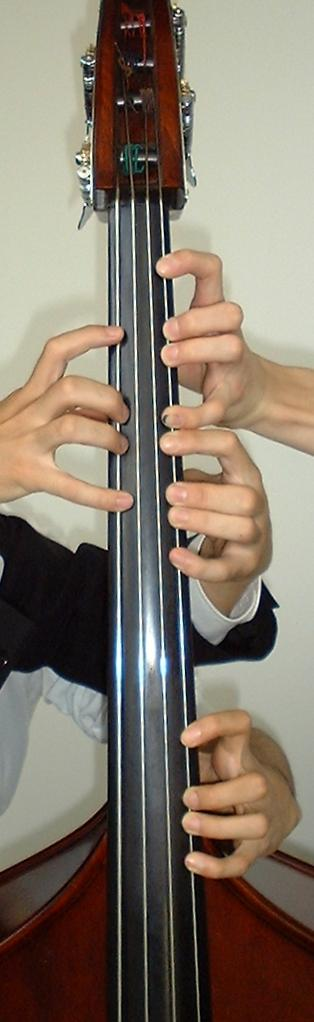
\includegraphics[height=7.5cm]{../Vol1/Pics/Position/4th_3.epsi}\\
{\flushleft\small 図\thefigure : 第IIIポジションは第IIと第IVの間\\}
\end{center}
\end{minipage}
\end{flushleft}

\subsection{音階練習 \label{3rd_scale}}
\begin{music}

\nostartrule
\parindent 0pt
\setclef1{\bass}  
\generalmeter{\meterC}
\generalsignature{2}    
\startpiece
\notes\zchar{14}{ニ長調(D-dur)音階}\enotes
\notes\zchar{19}{ニ長調(D-dur)音階}\enotes
\NOtes\zchar{14}{IV}\ovbkt{!e}{5.5}{3}\zchar{6}{\bf 0}\ql{'D}\zchar{7}{\bf 1}\ql{E}\zchar{8}{\bf 4}\ql{F}\zchar{9}{\bf 0}\ql{G}\enotes
\bar
\NOtes\zchar{10}{\bf 1}\ql{!a}\zchar{11}{\bf 4}\ql{b}\zchar{18}{III}\ovbkt{'c}{3.5}{0}\zchar{12}{\bf 2}\ql{!c}\zchar{13}{\bf 4}\ql{d}\enotes
\bar
\NOtes\zchar{13}{\bf 4}\ql{d}\zchar{12}{\bf 2}\ql{c}\zchar{11}{\bf 4}\zchar{17}{IV}\ovbkt{'b}{5.5}{-3}\ql{!b}\zchar{10}{\bf 1}\ql{a}\enotes
\bar
\NOtes\zchar{9}{\bf 0}\ql{'G}\zchar{8}{\bf 4}\ql{F}\zchar{7}{\bf 1}\ql{E}\zchar{6}{\bf 0}\ql{D}\enotes
\setdoublebar\endpiece
\setdoublebar\endpiece
\setclef1{\bass}  
\generalmeter{\meterC}
\generalsignature{3}    
\startpiece
\notes\zchar{14}{イ長調(A-dur)音階}\enotes
\NOtes\zchar{9}{\bf 0}\qu{'A}\zchar{9}{\bf 1}\qu{B}\zchar{9}{\bf 4}\qu{C}\zchar{9}{\bf 0}\ql{D}\enotes
\bar
\NOtes\zchar{9}{\bf 1}\ql{'E}\zchar{9}{\bf 4}\ql{F}\zchar{15}{III}\ovbkt{!g}{3.5}{0}\zchar{9}{\bf 2}\ql{'G}\zchar{10}{\bf 4}\ql{!a}\enotes
\bar
\NOtes\zchar{10}{\bf 4}\ql{!a}\zchar{9}{\bf 2}\ql{'G}\zchar{9}{\bf 4}\ql{F}\zchar{9}{\bf 1}\ql{E}\enotes
\bar
\NOtes\zchar{9}{\bf 0}\ql{'D}\zchar{9}{\bf 4}\qu{C}\zchar{9}{\bf 1}\qu{B}\zchar{9}{\bf 0}\qu{A}\enotes
\setdoublebar\endpiece
%\setclef1{\bass}  
%\generalmeter{\meterC}
%\generalsignature{-4}    
%\startpiece
%\notes\zchar{14}{変イ長調(As-dur)音階}\enotes
%\NOtes\zchar{9}{\bf 4}\qu{'A}\zchar{9}{\bf 1}\qu{B}\zchar{9}{\bf 2}\qu{C}\zchar{9}{\bf 4}\ql{D}\enotes
%\bar
%\NOtes\zchar{9}{\bf 1}\ql{'E}\zchar{9}{\bf 2}\ql{F}\zchar{9}{\bf 4}\ql{G}\zchar{10}{\bf 1}\ql{!a}\enotes
%\bar
%\NOtes\zchar{10}{\bf 1}\ql{!a}\zchar{9}{\bf 4}\ql{'G}\zchar{9}{\bf 2}\ql{F}\zchar{9}{\bf 1}\ql{E}\enotes
%\bar
%\NOtes\zchar{9}{\bf 4}\ql{'D}\zchar{9}{\bf 2}\qu{C}\zchar{9}{\bf 1}\qu{B}\zchar{9}{\bf 4}\qu{A}\enotes
%\setdoublebar\endpiece
%\setclef1{\bass}  
%\generalmeter{\meterC}
%\generalsignature{-5}    
%\startpiece
%\notes\zchar{14}{変ニ長調(Des-dur)音階}\enotes
%\NOtes\zchar{9}{\bf 4}\ql{'D}\zchar{9}{\bf 1}\ql{E}\zchar{9}{\bf 2}\ql{F}\zchar{9}{\bf 4}\ql{G}\enotes
%\bar
%\NOtes\zchar{10}{\bf 1}\ql{a}\zchar{11}{\bf 4}\ql{b}\zchar{12}{\bf 1}\ql{c}\zchar{13}{\bf 2}\ql{d}\enotes
%\bar
%\NOtes\zchar{13}{\bf 2}\ql{d}\zchar{12}{\bf 1}\ql{c}\zchar{11}{\bf 4}\ql{b}\zchar{10}{\bf 1}\ql{a}\enotes
%\bar
%\NOtes\zchar{9}{\bf 4}\ql{'G}\zchar{9}{\bf 2}\ql{F}\zchar{9}{\bf 1}\ql{E}\zchar{9}{\bf 4}\ql{D}\enotes
%\setdoublebar\endpiece
\end{music}

%\clearpage

\subsection{フラジオレット(伊: flageoletto)} 
弦長\footnote{弦の端から端までの長さ。通常1メートル強。}の中点は、軽く
触れるだけで開放弦の1オクターヴ上の音が出ます。これをフラジオレットと
呼びます\footnote{ハーモニクス(英: harmonics)とも呼ばれます。}。フラジ
オレットは弦長の\(\frac{1}{3}\)地点、\(\frac{1}{4}\)地点など、弦長
\(\frac{1}{n}\)($n$は2以上の自然数)の地点に存在します。

\clearpage

\subsection{調弦(英: tuning)}
3rdポジションは1の指が弦長の\(\frac{1}{4}\)地点、4の指が
\(\frac{1}{3}\)地点に位置しています。コンサートマスターのAの音に合わせ
て調弦するときには、コントラバスの調弦は3rdポジションが持つこの性質を
利用して行います。手順は以下の通りです。今日からチューニングメーターな
しでも調弦できるようにしましょう。

\begin{enumerate}
\item 4thポジションの1の指でD線を軽く押さえます。するとAの音が出る\footnote{弦長\(\frac{1}{3}\)地点なので開放弦の5度上の音が出ます。}ので、この音をコンサートマスターのAに合わせます。
\item 同じ位置を3rdポジションの4で取り直します。そして、1でA線のフラジオレット音\footnote{弦長\(\frac{1}{4}\)地点なので開放弦の2オクターヴ上の音が出ます。}を出します。この2つの音が同じピッチになるように調整します。
\item 左手を3rdポジションに置いたままで、A線の4とE線の1が同じピッチのフラジオレット音を出すように調整します。
\item 左手を3rdポジションに置いたままで、G線の4とD線の1が同じピッチのフラジオレット音を出すように調整します。これで4本の弦すべての調弦が完了します。
\end{enumerate}

演奏会本番では前もってチューニングメーターを用いて調弦をしておきましょう。舞台上で行う調弦は微調整程度で済ませるのが良いステージマナーです。

\subsection{第IIIポジションで弾く名曲}
\subsubsection*{シューベルト: ピアノ五重奏曲「ます」 第4楽章 第3変奏}
\begin{music}
\nostartrule
\startbarno=61
\def\writebarno{\tenrm\the\barno\barnoadd}
\def\raisebarno{2\internote}
\def\shiftbarno{0.1\Interligne}
\systemnumbers
\setclef1{\bass}
\generalsignature{2}    
\generalmeter{\meterfrac24}
\parindent 0pt
\startpiece\bigaccid
\notes\zchar{16}{\bf Var. III}\enotes
\Notes\zchar{-5}{II}\zchar{-8}{\p}\zchar{11}{\upbow}\zchar{8}{\bf 4}\lpz{'A}\cu{A}\enotes
\leftrepeat
\Notes\ibl{0}{'D}{0}\zchar{10}{\downbow}\zchar{8}{\bf 4}\upz{D}\qb{0}{D}\zchar{8}{\upbow}\upz{D}\qb{0}{D}\upz{F}\qb{0}{F}\tbl{0}\upz{F}\qb{0}{F}\enotes
\bar
\Notes\qu{'D}\qu{A}\enotes
\barno=62
\bar
\Notes\ibu{0}{'A}{0}\islurd{0}{A}\zchar{8}{\downbow}\qbp{0}{A}\tbbu{0}\tbu{0}\tslur{0}{!G}\lpz{'A}\qb{0}{A}\enotes
\Notes\ibbu{0}{'E}{-2}\islurd{0}{E}\zchar{-5}{III}\zchar{16}{\upbow}\zchar{13}{\bf 4}\qbp{0}{E}\tbbbu{0}\zchar{13}{\bf 1}\qb{0}{D}\zchar{-5}{I}\zchar{12}{\bf 4}\qbp{0}{C}\tbbbu{0}\tbbu{0}\tbu{0}\tslur{0}{B}\zchar{12}{\bf 1}\qb{0}{B}\enotes
\bar
\Notes\zchar{-4}{II}\zchar{11}{\downbow}\zchar{8}{\bf 4}\qu{'A}\enotes
\notes\ds\zchar{8}{\upbow}\cu{'A}\enotes
\bar
\Notes\ibl{0}{'D}{0}\zchar{8}{\downbow}\upz{D}\qb{0}{D}\zchar{8}{\upbow}\upz{D}\qb{0}{D}\upz{F}\qb{0}{F}\tbl{0}\upz{F}\qb{0}{F}\enotes
\bar
\Notes\ql{'D}\ibu{0}{C}{4}\islurd{0}{!G}\lpz{'A}\qb{0}{A}\tbu{0}\tslur{0}{C}\zchar{-4}{III}\lpz{D}\zchar{12}{\bf 1}\qb{0}{D}\enotes
\bar
\Notes\zchar{10}{\downbow}\zchar{8}{\bf 4}\cl{'E}\ds\zchar{8}{\upbow}\cl{E}\ds\enotes
\bar
\Notes\zchar{8}{\downbow}\qup{'A}\zchar{8}{\upbow}\cu{A}\enotes
\rightrepeat
\Notes\ibu{0}{'C}{0}\zchar{-5}{II}\zchar{12}{\downbow}\zchar{10}{\bf 2}\lpz{C}\qb{0}{C}\tbu{0}\zchar{10}{\upbow}\lpz{C}\qb{0}{C}\enotes
\notes\ibbu{0}{'B}{0}\islurd{0}{D}\zchar{13}{\downbow}\zchar{11}{\bf 4}\qb{0}{D}\zchar{11}{\bf 2}\qb{0}{C}\zchar{-5}{I}\zchar{11}{\bf 1}\qb{0}{B}\tbbu{0}\tbu{0}\tslur{0}{C}\zchar{-5}{II}\zchar{11}{\bf 2}\qb{0}{C}\enotes
\bar
\Notes\islurd{0}{'D}\zchar{13}{\upbow}\zchar{10}{\bf 4}\qu{D}\tslur{0}{A}\zchar{8}{\bf 4}\cu{A}\zchar{13}{\upbow}\zchar{10}{\bf 4}\cu{D}\enotes
\bar
\Notes\ibu{0}{'C}{0}\lpz{C}\qb{0}{C}\tbu{0}\lpz{C}\qb{0}{C}\enotes
\notes\ibbl{0}{'E}{0}\isluru{0}{E}\qb{0}{C}\midslur{3}\qb{0}{G}\zchar{-7}{I}\zchar{10}{\bf 1}\qb{0}{E}\tbbl{0}\tbl{0}\tslur{0}{C}\zchar{-7}{II}\zchar{9}{\bf 2}\qb{0}{C}\enotes
\bar
\Notes\islurd{0}{'D}\zchar{13}{\upbow}\zchar{10}{\bf 4}\qu{D}\tslur{0}{`D}\cu{D}\zchar{10}{\upbow}\cu{'D}\enotes
\bar
\Notes\ibu{0}{'B}{2}\zchar{-5}{III}\zchar{12}{\downbow}\zchar{10}{\bf 4}\qb{0}{B}\zchar{10}{\upbow}\qb{0}{BB}\tbu{0}\zchar{11}{\bf 1}\qb{0}{D}\enotes
\bar
\Notes\islurd{0}{'D}\zchar{11}{\downbow}\lsf{A}\qu{D}\tslur{0}{A}\zchar{8}{\bf 1}\cu{A}\zchar{9}{\upbow}\cu{A}\enotes
\bar
\Notes\ibu{0}{'A}{0}\zchar{8}{\downbow}\qbp{0}{A}\tbbu{0}\tbu{0}\zchar{8}{\upbow}\qb{0}{A}\ibu{0}{E}{-4}\zchar{14}{\downbow}\zchar{12}{\bf 4}\qb{0}{E}\tbu{0}\zchar{-5}{II}\zchar{14}{\upbow}\zchar{11}{\bf 2}\qb{0}{C}\enotes
\bar
\Notes\islurd{0}{'D}\zchar{11}{\downbow}\qu{D}\tslur{0}{`D}\cu{D}\zchar{10}{\upbow}\cu{'D}\enotes
\bar
\Notes\ibu{0}{'B}{2}\zchar{-5}{III}\zchar{10}{\bf 4}\qb{0}{BBB}\tbu{0}\zchar{12}{\bf 1}\qb{0}{D}\enotes
\bar
\Notes\islurd{0}{'D}\usf{!b}\qu{'D}\tslur{0}{A}\zchar{8}{\bf 1}\cu{A}\cu{A}\enotes
\bar
\Notes\ibu{0}{'A}{0}\qbp{0}{A}\tbbu{0}\tbu{0}\qb{0}{A}\ibu{0}{E}{-4}\zchar{12}{\bf 4}\qb{0}{E}\tbu{0}\zchar{-5}{II}\zchar{12}{\bf 2}\qb{0}{C}\enotes
\bar
\Notes\qlp{'D}\enotes
\mulooseness=0
\setdoublebar\endpiece
\end{music}
